%=== CHAPTER THREE (3) ===
%=== (Actual work done and contribution, including literature survey) ===

\chapter{Methods}
\begin{spacing}{1.5}
\setlength{\parskip}{0.3in}
%  (Actual work done and contribution, including literature survey)


\section{Skin Chromophore Color Space Decomposition}
In digital photos, skin color represents only a small subset of the sRGB space, due to unique chromophores contained in the skin, such as melanin and heamoglobin, which give the skin a unique and limited color range. However, finding a transformation from sRGB values to the absolute concentration of skin chromophores is challenging, as the sRGB color space is device-agnostic. It also requires calibrating the camera system using pigmentation data in vivo. This issue is bypassed by modeling the \textit{relative} pigment concentration against the base skin, so that the transformed color space can well express the influence of different chromophores on skin color without the need for camera system calibration.

Specifically, the relative absorption of incident light by the chromophore can be described by the Beer-Lambert law, namely:
\begin{equation}
    A(\lambda) = -log(R(\lambda)) = C\epsilon l,
    \label{eq1}
\end{equation}
where $A$ represents absorption, $R$ is the reflection intensity, $\lambda$ is the wavelengths, $C$ is the relative concentration, $\epsilon$ denotes the extinction coefficient of chromophore and $l$ is the mean optical path length.

In this work, the impact of two chromophores on the skin, melanin and heamoglobin, and a residual term, are mainly considered, as shown in Figure \ref{fig:skin_model}. Therefore,
\begin{equation}
    A(\lambda) = C_H\epsilon_H(\lambda)l_H + C_M\epsilon_M(\lambda)l_M + C_r\epsilon_r(\lambda)l_r,
    \label{eq2}
\end{equation}
where subscript $H$, $M$, and $r$ represent heamoglobin, melanin, and residual chromophore, respectively.

In this method, log-RGB values are used as the approximation of real reflection intensity $R$. Although pixel intensity does not fully reflect the real case, it is sufficient to estimate the pigment concentration ratio of pigmentations relative to base skin. Considering the response of each chromophore under the three camera pixel channels R, G, and B, Equations \ref{eq1} and \ref{eq2} can be written as:
\begin{equation}
    \begin{aligned}
         & C_H\epsilon_H^c l_H + C_M\epsilon_M^c l_M + C_r\epsilon_r^c l_r = -log(R^c) \\
         & c\in\{\mathcal{R},\mathcal{G},\mathcal{B}\},
    \end{aligned}
\end{equation}
or in matrix form
\begin{gather*}
    \mathbf{E}\mathbf{c}=-log(\mathbf{k}),\\
    \mathbf{E}=\begin{bmatrix}
        \epsilon_H^\mathcal{R} l_H & \epsilon_M^\mathcal{R} l_M & \epsilon_r^\mathcal{R} l_r \\
        \epsilon_H^\mathcal{G} l_H & \epsilon_M^\mathcal{G} l_M & \epsilon_r^\mathcal{G} l_r \\
        \epsilon_H^\mathcal{B} l_H & \epsilon_M^\mathcal{B} l_M & \epsilon_r^\mathcal{B} l_r
    \end{bmatrix},\
    \mathbf{c}=\begin{bmatrix}C_H \\C_M \\C_r\end{bmatrix},\
    \mathbf{k}=\begin{bmatrix}R^\mathcal{R} \\R^\mathcal{G} \\R^\mathcal{B}\end{bmatrix}.
\end{gather*}

Following the practice of Tsumura et al.\cite{tsumura1999independent}, $E$ is estimated by Fast Independent Component Analysis(FastICA)\cite{HYVARINEN2000411} in the log-RGB domain. Specifically, 128 patches are randomly sampled from each face skin image of the dataset, and each patch is 16x16 pixels in size. Then the average RGB value of each patch is calculated. The FastICA algorithm in \texttt{sklearn}\cite{scikit-learn} is adopted to estimate the 3 independent components over the log-RGB domain as $\mathbf{E}$. In this work, $\hat{\mathbf{E}}$ is obtained as follows:
\begin{equation}
    \hat{\mathbf{E}} = \begin{bmatrix}
        0.96  & -0.63 & 0.9  \\
        -0.22 & 0.35  & 0.17 \\
        -0.16 & -0.69 & -0.4 \\
    \end{bmatrix}
\end{equation}

\section{Spot Appearance Modelling Based on Sum-of-Gaussians}
The proposed method is based on the observation that pigmentation and acne of interest tend to have blurred edges. On one hand, they are caused by local accumulation of chromophores under the skin due to various stressors such as UV or inflammation, which can be modeled as Gaussian distributions. On the other hand, subsurface scattering of light under the skin makes pigmentation look even blurry. With Gaussian functions, both phenomena can be described very well, because the convolution of two Gaussian functions is still a Gaussian function, namely:
\begin{equation}
    \begin{aligned}
         & G(x; \mu_a, \sigma_a, A)\star G(x; \mu_b, \sigma_b, B)                 \\
         & \qquad= A\cdot B\cdot G(x; \mu_a+\mu_b, \sqrt{\sigma_a^2+\sigma_b^2}),
    \end{aligned}
\end{equation}
where $\star$ is the convolution operator, and Gaussian function $G$ is defined as
\begin{equation}
    G(x; \mu, \sigma, A) = \frac{A}{\sigma\sqrt{2\pi}}e^{-\frac{{(x - \mu)^2}}{{2\sigma^2}}},
\end{equation}
and this conclusion can also be generalized to multivariate Gaussian functions.

Existing fast subsurface scattering implementations are followed, using multiple Gaussian functions to approximate the appearance of a blemish under the scattering skin tissue. First, a generalized 2D Gaussian function is defined as

\begin{equation}
    \begin{aligned}
         & G^\prime(x, y; \mu_x, \mu_y, \sigma_x, \sigma_y, \theta, A)                                                                                 \\
         & \qquad=\frac{A}{2\pi \sigma_x \sigma_y}\cdot e^{-\frac{{(x' - \mu_x)^2}}{{2 \sigma_x^2}} - \frac{{(y' - \mu_y)^2}}{{2 \sigma_y^2}}},\ where \\
         & x' = x \cos\theta - y \sin\theta,                                                                                                           \\
         & y' = x \sin\theta + y \cos\theta.
    \end{aligned}
\end{equation}

Compared to the standard 2D Gaussian function, a rotation parameter $\theta$ is added to allow $G^\prime$ to rotate. It enables modeling more complex situations. In the implementation, $\theta$ is fixed for all Gaussian functions to be summed, which ensures that the assumptions hold. The relative chromophore concentration of each distribution is thus defined as a sum of 3 or more $G^\prime$s (note that $\theta$ is the same for all $G^\prime$s), namely:
\begin{equation}
    \begin{aligned}
         & \hat{C_K}(x,y) = \sum_{i=1}^{N}G_i^\prime(x, y; \mu_x^i, \mu_y^i, \sigma_x^i, \sigma_y^i, \theta, A_i), \\
         & K\in\{H,M,r\},\quad N\ge3.
    \end{aligned}
\end{equation}

The parameters are fitted by the Levenberg-Marquardt method\cite{10.1007/BFb0067700} with the \texttt{lmfit} Python library\cite{newville_matthew_2014_11813}. After successful fitting of $\hat{C_K}$s, they are simply multiplied with user-input control parameters $\alpha_K$ to amplify/attenuate the intensity of chromophore channels. Thus, the relative reflection of a modified pigmentation can be written as
\begin{gather*}
    -log(\mathbf{k}^\prime) = \mathbf{E}\mathbf{A}\hat{\mathbf{c}},\\
    \mathbf{A}=diag(\alpha_H, \alpha_M, \alpha_r),\quad
    \hat{\mathbf{c}} = [\hat{C_H}, \hat{C_M}, \hat{C_r}]^T.
\end{gather*}


\begin{figure}[t]
    \centering
    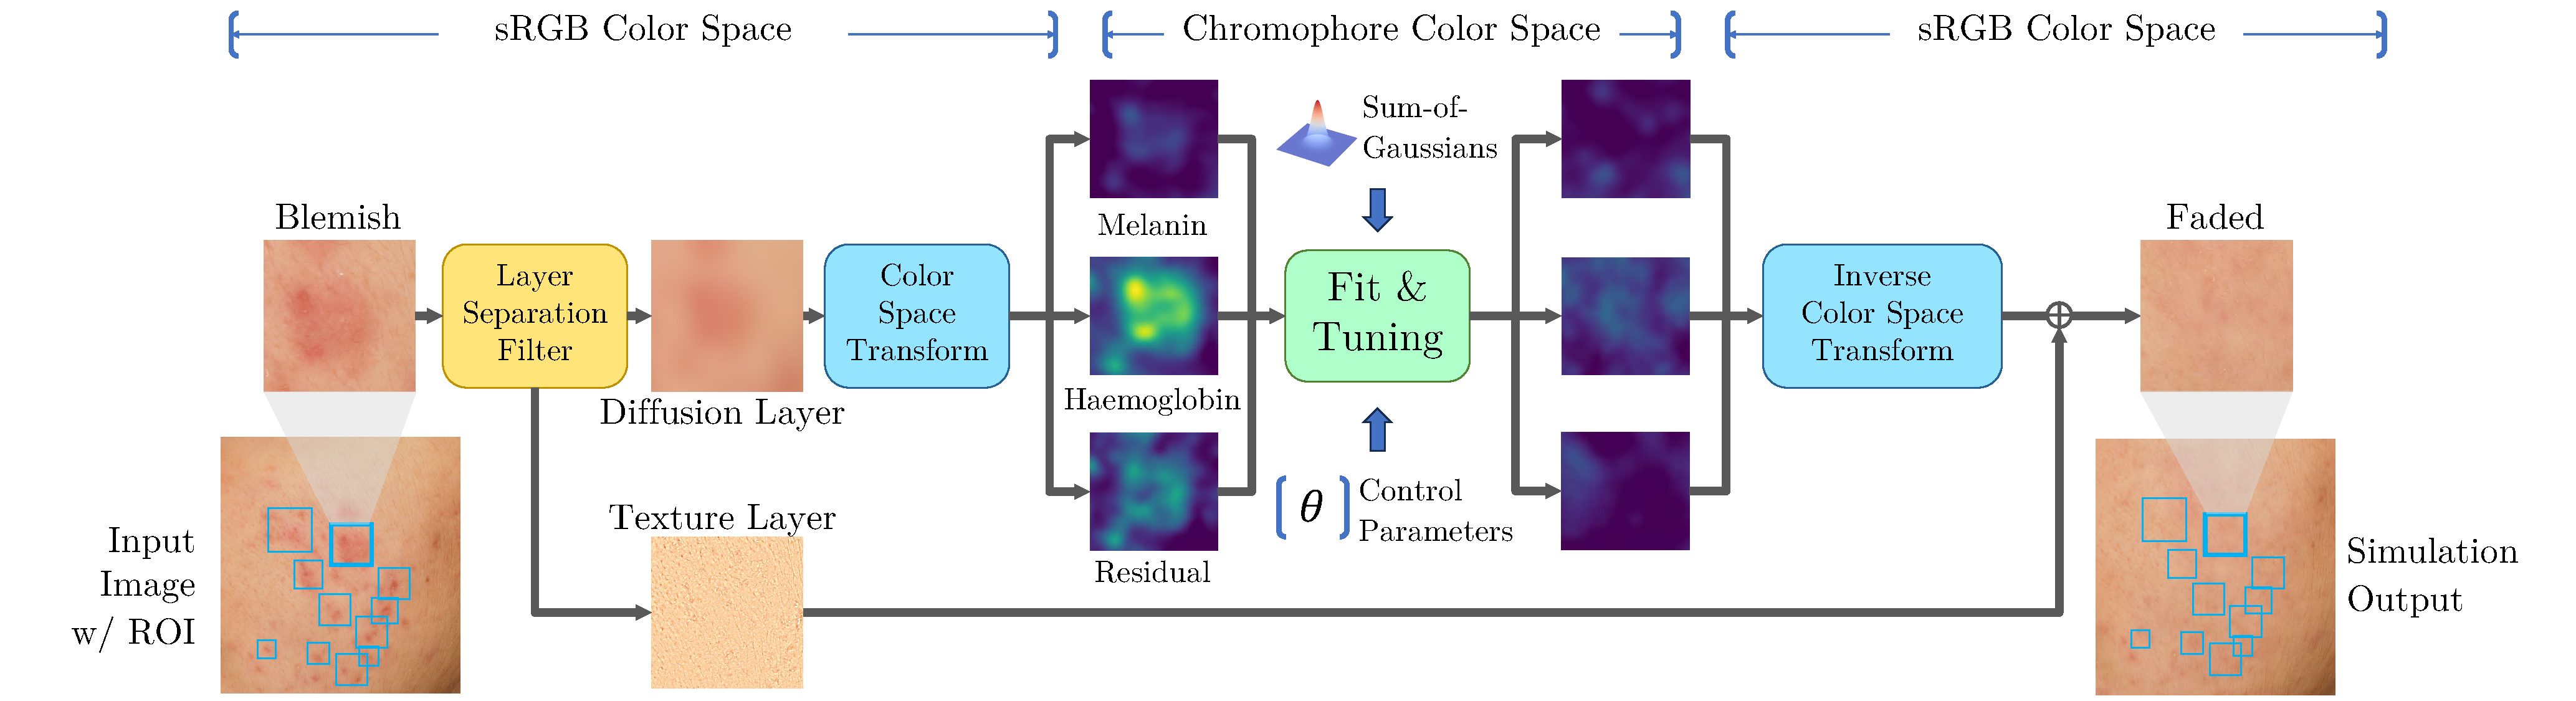
\includegraphics[width=0.94\columnwidth]{Chapter3/system.pdf}
    \caption{An overview of the proposed skin blemish change simulation pipeline. In the pipeline, a box of Region of Interest (ROI) is first used to select the blemish like acne or pigmentation. Then, a \textit{Layer Separation Filter} is applied to separate the texture layer and the diffusion layers. A \textit{Sum-of-Gaussians} model is fitted to each ROI in \textit{Melanin/Heamoglobin} color space, with the parameters of the fitted model adjusted to manipulate the appearance of the blemishes. The modified diffusion layer is summed with the original texture layer to obtain the output.}
    \label{fig:system}
\end{figure}
\subsection{Algorithm Implementations}

As shown in Figure \ref{fig:system}, in the pipeline, a skin layer separation filter is first adopted to separate the skin into a surface texture layer (including specular reflections and skin textures) and a scattered chromophore layer. This is implemented using a Gaussian filter with a small variance, small enough to isolate the detail texture of the skin without affecting the underlying assumptions. Then, the image is converted from sRGB to log-RGB space (assuming the image is scaled to $[0,1]$ and with no Gamma correction).

A simple GUI is also created to allow users to draw bonding boxes or upload a segmentation map to select desired spots. Then, each spot is fitted and control parameters are applied for each pigmentation channel. After that, the inverse color space transform is applied and the texture layer, bypassed from the input, is added to the modified chromophore layer.

In the actual implementation, several optimizations are performed to the program:
\begin{itemize}
    \item Each channel and each spot can be fitted independently. Multi-process parallelism is used to speed this up.
    \item Since $\hat{C_K}$ has explicit partial derivatives, the Jacobian matrix is manually derived. This assists the fitting procedure to quickly compute accurate gradients rather than estimate them numerically.
    \item Although the entire Sum-of-Gaussians model could be fitted at once, the convergence of the fit would be slow. Therefore, a strategy is adopted where a new $N$-th Gaussian function is gradually introduced into the model with $N-1$ functions and the updated model is fitted, during which the existing parameters are frozen. Finally, all parameters are unfrozen for one more fitting as a fine-tuning. In this way, only one function is fitted each time except for the last one.
\end{itemize}

This algorithm can be represented by the following pseudocode.
\begin{algorithm}
    \caption{Fitting Distribution of a Spot}
    \begin{algorithmic}[1]
    
    \State \textbf{Input:} Spot image patch $X\in\mathbb{R}^3$ from user input
    
    \State \textbf{Preprocessing:}
    % \Indent
        \State $X \gets \gamma^{-1}(X/255.0)$ \Comment{Inverse gamma transformation to linear RGB space}
        \State $X \gets \mathbf{E}^{-1}\cdot\log{X}$ \Comment{Transform to chromophore color space}
    % \EndIndent
    
    \For{each channel $c$ in \{H, M, r\}}
        \State Initialize empty base model $\hat{C_K}(x, y)$
        \For{each Gaussian component $G_i$}
            \State Estimate initial center position $x^{init}_i, y^{init}_i$
            \State Fit $G_i^c(x, y; \mu_x^i, \mu_y^i, \sigma_x^i, \sigma_y^i, \theta, A_i)$
            \State $\hat{C_K} \gets \hat{C_K}+G_i^c$
            \State Freeze parameters of $\hat{C_K}$
        \EndFor
        \State Unfreeze all parameters for final refinement fit
    \EndFor
    
    \State \textbf{Return:} Fitted parameters and fitted spot image
    
    \end{algorithmic}
    \end{algorithm}

%=== END OF CHAPTER THREE ===
\end{spacing}
\newpage
